\subsection*{Minimum Spanning Tree}

To create the minimum spanning tree (MST), iterate through the edges (in order of weight -- Kruskal's Algorithm), taking into consideration only edges with the weight of the current wave (e.g., 1, 2, 3, \ldots). The edge is a member of the MST if and only if the edge can be added to the MST without creating a cycle (a closed area within the graph). \\

\begin{enumerate}
 \item[Wave 1]
\begin{center}
\adjustbox{valign=t}{
\begin{tikzpicture}[auto,node distance=2.5cm,main node/.style={circle,draw}]
  \node[main node] (1) {1};
  \node[main node] (2) [below right of=1] {2};
  \node[main node] (3) [above right of=2] {3};
  \node[main node] (4) [above right of=3] {4};
  \node[main node] (5) [below right of=3] {5};
  \node[main node] (6) [below right of=4] {6};
  \node[main node] (7) [below right of=6] {7};
  \node[main node] (8) [above right of=7] {8};
  \node[main node] (9) [above right of=1] {9};
  
  \path[line width=1.2pt, every node/.style={font=\small}]
    (3) edge node [right] {1} (4)
    (7) edge node [right] {1} (8);
\end{tikzpicture} 
} \\[3em]
\end{center} 

 \item[Wave 2]
\begin{center}
\adjustbox{valign=t}{
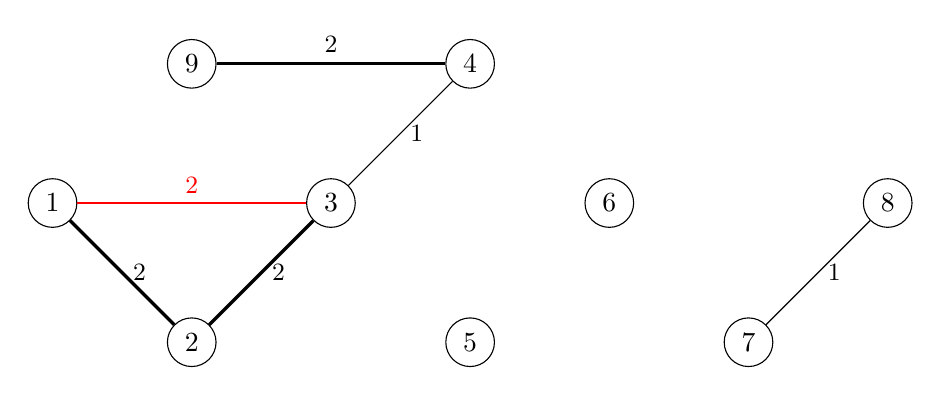
\begin{tikzpicture}[auto,node distance=2.5cm,main node/.style={circle,draw}]
  \node[main node] (1) {1};
  \node[main node] (2) [below right of=1] {2};
  \node[main node] (3) [above right of=2] {3};
  \node[main node] (4) [above right of=3] {4};
  \node[main node] (5) [below right of=3] {5};
  \node[main node] (6) [below right of=4] {6};
  \node[main node] (7) [below right of=6] {7};
  \node[main node] (8) [above right of=7] {8};
  \node[main node] (9) [above right of=1] {9};
  
  \path[every node/.style={font=\small}]
    (3) edge node [right] {1} (4)
    (7) edge node [right] {1} (8);
    
  \path[line width=1.2pt, every node/.style={font=\small}]
    (1) edge node [right] {2} (2)
    (2) edge node [right] {2} (3)
    (9) edge node [above] {2} (4);
    
  \path[color=red, every node/.style={font=\small, color=red}]
    (1) edge node [above] {2} (3);
\end{tikzpicture}
} \\[3em]
\end{center}

\item[Wave 3]
\begin{center}
\adjustbox{valign=t}{
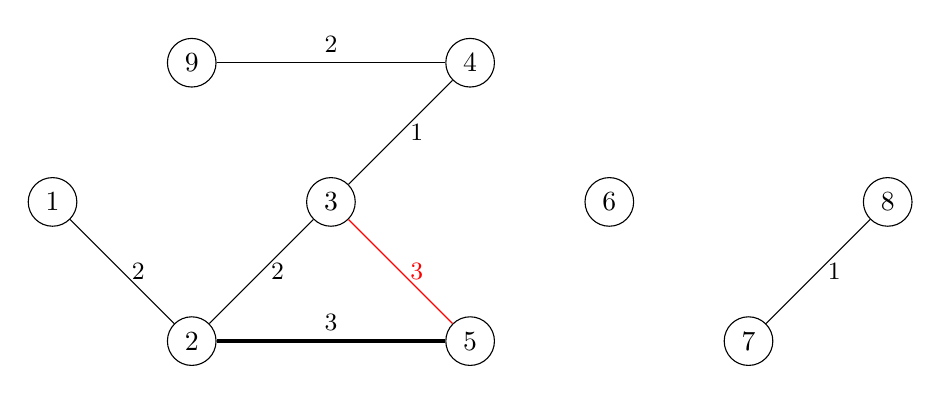
\begin{tikzpicture}[auto,node distance=2.5cm,main node/.style={circle,draw}]
  \node[main node] (1) {1};
  \node[main node] (2) [below right of=1] {2};
  \node[main node] (3) [above right of=2] {3};
  \node[main node] (4) [above right of=3] {4};
  \node[main node] (5) [below right of=3] {5};
  \node[main node] (6) [below right of=4] {6};
  \node[main node] (7) [below right of=6] {7};
  \node[main node] (8) [above right of=7] {8};
  \node[main node] (9) [above right of=1] {9};
  
  \path[every node/.style={font=\small}]
    (3) edge node [right] {1} (4)
    (7) edge node [right] {1} (8)
    (1) edge node [right] {2} (2)
    (2) edge node [right] {2} (3)
    (9) edge node [above] {2} (4);
    
  \path[line width=1.2pt, every node/.style={font=\small}]
    (2) edge node [above] {3} (5);
    
  \path[color=red, every node/.style={font=\small, color=red}]
    (5) edge node [right] {3} (3);
\end{tikzpicture}
} \\[3em]
\end{center}

\item[Wave 4]
\begin{center}
\adjustbox{valign=t}{
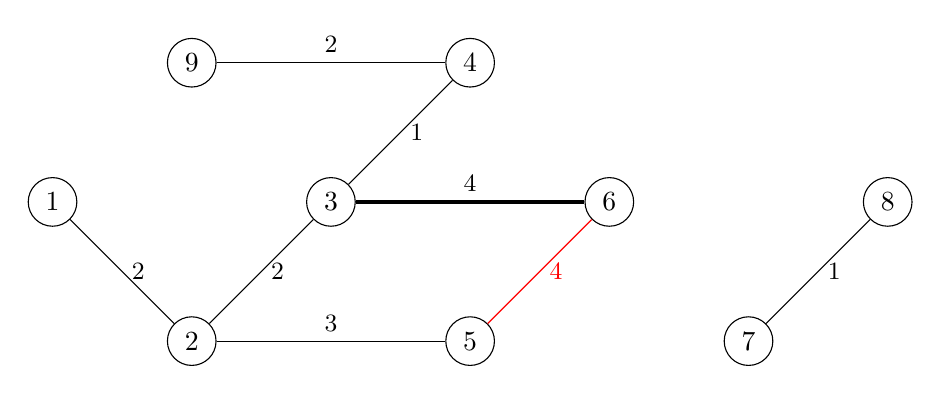
\begin{tikzpicture}[auto,node distance=2.5cm,main node/.style={circle,draw}]
  \node[main node] (1) {1};
  \node[main node] (2) [below right of=1] {2};
  \node[main node] (3) [above right of=2] {3};
  \node[main node] (4) [above right of=3] {4};
  \node[main node] (5) [below right of=3] {5};
  \node[main node] (6) [below right of=4] {6};
  \node[main node] (7) [below right of=6] {7};
  \node[main node] (8) [above right of=7] {8};
  \node[main node] (9) [above right of=1] {9};
  
  \path[every node/.style={font=\small}]
    (3) edge node [right] {1} (4)
    (7) edge node [right] {1} (8)
    (1) edge node [right] {2} (2)
    (2) edge node [right] {2} (3)
    (9) edge node [above] {2} (4)
    (2) edge node [above] {3} (5);
    
  \path[line width=1.2pt, every node/.style={font=\small}]
    (3) edge node [above] {4} (6);
    
  \path[color=red, every node/.style={font=\small, color=red}]
    (5) edge node [right] {4} (6);
\end{tikzpicture}
} \\[3em]
\end{center}

\item[Wave 5]
\begin{center}
\adjustbox{valign=t}{
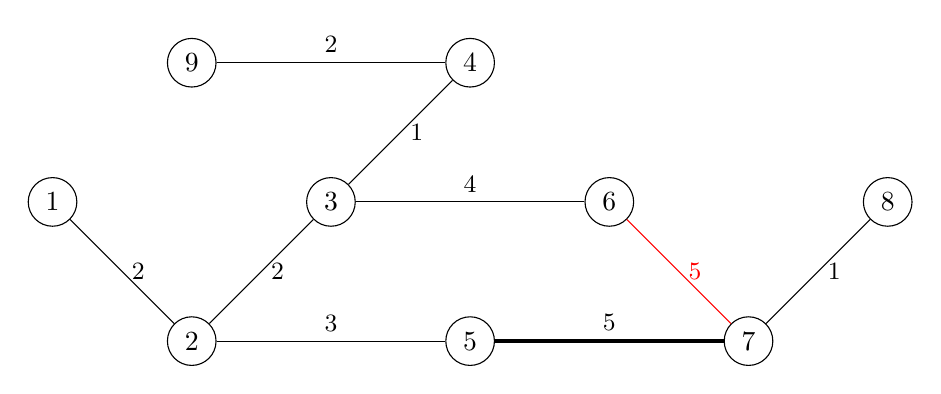
\begin{tikzpicture}[auto,node distance=2.5cm,main node/.style={circle,draw}]
  \node[main node] (1) {1};
  \node[main node] (2) [below right of=1] {2};
  \node[main node] (3) [above right of=2] {3};
  \node[main node] (4) [above right of=3] {4};
  \node[main node] (5) [below right of=3] {5};
  \node[main node] (6) [below right of=4] {6};
  \node[main node] (7) [below right of=6] {7};
  \node[main node] (8) [above right of=7] {8};
  \node[main node] (9) [above right of=1] {9};
  
  \path[every node/.style={font=\small}]
    (3) edge node [right] {1} (4)
    (7) edge node [right] {1} (8)
    (1) edge node [right] {2} (2)
    (2) edge node [right] {2} (3)
    (9) edge node [above] {2} (4)
    (2) edge node [above] {3} (5)
    (3) edge node [above] {4} (6);
    
  \path[line width=1.2pt, every node/.style={font=\small}]
    (5) edge node [above] {5} (7);
    
  \path[color=red, every node/.style={font=\small, color=red}]
    (6) edge node [right] {5} (7);
\end{tikzpicture}
} \\[3em]
\end{center}

\item[Wave 6]
\begin{center}
\adjustbox{valign=t}{
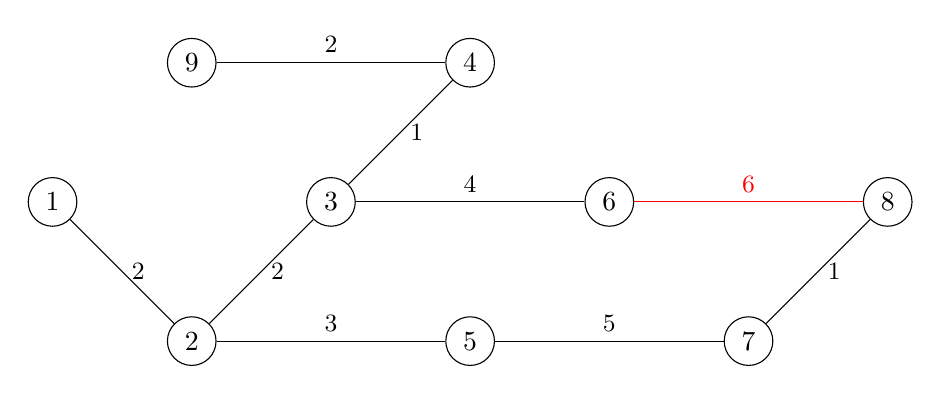
\begin{tikzpicture}[auto,node distance=2.5cm,main node/.style={circle,draw}]
  \node[main node] (1) {1};
  \node[main node] (2) [below right of=1] {2};
  \node[main node] (3) [above right of=2] {3};
  \node[main node] (4) [above right of=3] {4};
  \node[main node] (5) [below right of=3] {5};
  \node[main node] (6) [below right of=4] {6};
  \node[main node] (7) [below right of=6] {7};
  \node[main node] (8) [above right of=7] {8};
  \node[main node] (9) [above right of=1] {9};
  
  \path[every node/.style={font=\small}]
    (3) edge node [right] {1} (4)
    (7) edge node [right] {1} (8)
    (1) edge node [right] {2} (2)
    (2) edge node [right] {2} (3)
    (9) edge node [above] {2} (4)
    (2) edge node [above] {3} (5)
    (3) edge node [above] {4} (6)
    (5) edge node [above] {5} (7);
    
  \path[color=red, every node/.style={font=\small, color=red}]
    (6) edge node [above] {6} (8);
\end{tikzpicture}
} \\[3em]
\end{center}

\item[Wave 7]
\begin{center}
\adjustbox{valign=t}{
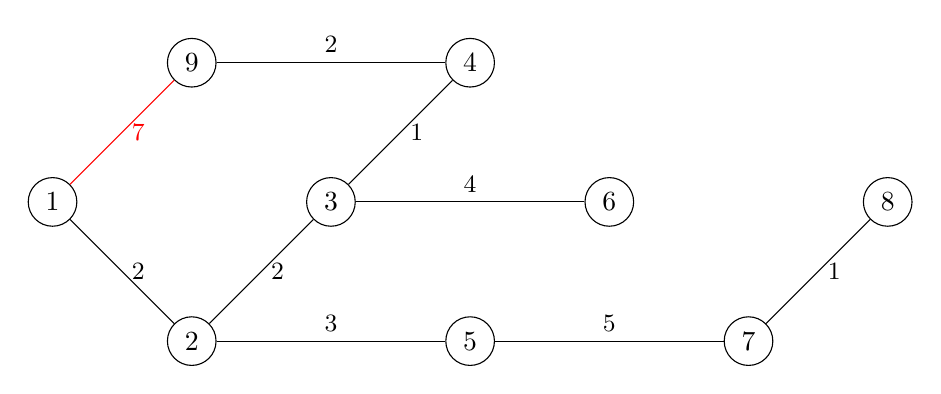
\begin{tikzpicture}[auto,node distance=2.5cm,main node/.style={circle,draw}]
  \node[main node] (1) {1};
  \node[main node] (2) [below right of=1] {2};
  \node[main node] (3) [above right of=2] {3};
  \node[main node] (4) [above right of=3] {4};
  \node[main node] (5) [below right of=3] {5};
  \node[main node] (6) [below right of=4] {6};
  \node[main node] (7) [below right of=6] {7};
  \node[main node] (8) [above right of=7] {8};
  \node[main node] (9) [above right of=1] {9};
  
  \path[every node/.style={font=\small}]
    (3) edge node [right] {1} (4)
    (7) edge node [right] {1} (8)
    (1) edge node [right] {2} (2)
    (2) edge node [right] {2} (3)
    (9) edge node [above] {2} (4)
    (2) edge node [above] {3} (5)
    (3) edge node [above] {4} (6)
    (5) edge node [above] {5} (7);
    
  \path[color=red, every node/.style={font=\small, color=red}]
    (1) edge node [right] {7} (9);
\end{tikzpicture}
} \\[3em]
\end{center}

\item[Final]
\begin{figure}[H]
\begin{center}
\adjustbox{valign=t}{
\begin{tikzpicture}[auto,node distance=2.5cm,main node/.style={circle,draw}]
  \node[main node] (1) {1};
  \node[main node] (2) [below right of=1] {2};
  \node[main node] (3) [above right of=2] {3};
  \node[main node] (4) [above right of=3] {4};
  \node[main node] (5) [below right of=3] {5};
  \node[main node] (6) [below right of=4] {6};
  \node[main node] (7) [below right of=6] {7};
  \node[main node] (8) [above right of=7] {8};
  \node[main node] (9) [above right of=1] {9};
  
  \path[every node/.style={font=\small}]
    (3) edge node [right] {1} (4)
    (7) edge node [right] {1} (8)
    (1) edge node [right] {2} (2)
    (2) edge node [right] {2} (3)
    (9) edge node [above] {2} (4)
    (2) edge node [above] {3} (5)
    (3) edge node [above] {4} (6)
    (5) edge node [above] {5} (7);
\end{tikzpicture}
} \\[10pt]
\end{center}
\caption{Minimum Spanning Tree}
\end{figure}

\end{enumerate}